% !TeX spellcheck = hu_HU
% !TeX encoding = UTF-8
% !TeX program = xelatex
\documentclass[11pt,a4paper,oneside]{report}             % Single-side
%\documentclass[11pt,a4paper,twoside,openright]{report}  % Duplex

\input{include/packages}

%TODO Set the main variables
\newcommand{\vikszerzoVezeteknev}{Király}
\newcommand{\vikszerzoKeresztnev}{Bálint Martin}

\newcommand{\vikkonzulensAMegszolitas}{}
\newcommand{\vikkonzulensAVezeteknev}{Schulcz}
\newcommand{\vikkonzulensAKeresztnev}{Róbert}

\newcommand{\vikkonzulensBMegszolitas}{}
\newcommand{\vikkonzulensBVezeteknev}{}
\newcommand{\vikkonzulensBKeresztnev}{}

\newcommand{\vikkonzulensCMegszolitas}{}
\newcommand{\vikkonzulensCVezeteknev}{}
\newcommand{\vikkonzulensCKeresztnev}{}

\newcommand{\vikcim}{Leltározási feladatokat segítő, grafikus felülettel rendelkező adatbázis tervezése és fejlesztése} % Cím
\newcommand{\viktanszek}{\bmehit} % Tanszék
\newcommand{\vikdoktipus}{\bsc} % Dokumentum típusa (\bsc vagy \msc)
\newcommand{\vikmunkatipusat}{szakdolgozatot} % a "hallgató nyilatkozat" részhez: szakdolgozatot vagy diplomatervet

\input{include/tdk-variables}
\newcommand{\szerzoMeta}{\vikszerzoVezeteknev{} \vikszerzoKeresztnev} % egy szerző esetén

\input{include/thesis-hu}

\input{include/preamble}

%--------------------------------------------------------------------------------------
% Table of contents and the main text
%--------------------------------------------------------------------------------------
\begin{document}

\pagenumbering{gobble}
\nocite{*}

\include{include/project}

\selectthesislanguage


\makeatletter

\renewcommand*{\ext@figure}{lot}

\let\c@figure\c@table

\let\ftype@figure\ftype@table

\let\listoftableandfigures\listoftables

\renewcommand*\listtablename{List of Tables and figures}

\makeatother

%TODO Titlepage
%~~~~~~~~~~~~~~~~~~~~~~~~~~~~~~~~~~~~~~~~~~~~~~~~~~~~~~~~~~~~~~~~~~~~~~~~~~~~~~~~~~~~~~
\include{include/titlepage}		   % Szakdolgozat/Diplomaterv címlap

% Table of Contents
%~~~~~~~~~~~~~~~~~~~~~~~~~~~~~~~~~~~~~~~~~~~~~~~~~~~~~~~~~~~~~~~~~~~~~~~~~~~~~~~~~~~~~~
\tableofcontents\vfill


% Declaration and Abstract
%~~~~~~~~~~~~~~~~~~~~~~~~~~~~~~~~~~~~~~~~~~~~~~~~~~~~~~~~~~~~~~~~~~~~~~~~~~~~~~~~~~~~~~
\include{include/declaration} %TODO Hallgatói nyilatkozat -- TDK és OTDK esetén törlendő!
% !TeX spellcheck = hu_HU
\pagenumbering{roman}
\setcounter{page}{1}

\selecthungarian

%----------------------------------------------------------------------------
% Abstract in Hungarian
%----------------------------------------------------------------------------
\chapter*{Kivonat}\addcontentsline{toc}{chapter}{Kivonat}

Rengeteg raktárkezelő alkalmazás érhető el a piacon, azonban a térképes nézet egy ritka funkciónak számít ezekben a rendszerekben. Az erre alkalmas szoftverek rendszerint előredefiniált térképpel dolgoznak.

A szakdolgozatom célja egy olyan raktár kezelő rendszer tervezése és fejlesztése, amely lehetővé teszi az eszközök pozíciójának pontos meghatározását a raktáron belül, mindezt dinamikusan. A rendszer segítségével a felhasználók képesek a raktár méretét és elrendezését is meghatározni, így a pontos igényeknek megfelelő alkalmazást kaphatnak.

A feladat megvalósítása során kutatást végeztem a meglévő rendszerekről, majd elkészítettem a feladat specifikációt, valamint az alkalmazás wireframe-eit. Ezek definiálása után elkezdtem az architekturális tervezést, majd neki láttam az alkalmazás implementálásának. Az üzleti logikát és a kliens oldali megjelenítést is JavaScript, pontosabban annak egy superset-jével, a TypeScript-tel valósítottam meg. A fejlesztés után és közben teszteket készítettem a működés ellenőrzése érdekében.

\vfill
\selectenglish

%----------------------------------------------------------------------------
% Abstract in English
%----------------------------------------------------------------------------
\chapter*{Abstract}\addcontentsline{toc}{chapter}{Abstract}

There is a great deal of warehouse management applications available in the market, however, the map view is a rare feature in these systems. The warehouse management software usually works with a predefined maps.

The aim of my dissertation is to design and develop a warehouse management system that allows to determine the exact position of items within the warehouse. With the help of the system, users can also set the size and layout of the warehouse, so they can get the application that suits their exact needs.

During the implementation of the task, I conducted research on the existing systems and then prepared the task specification as well as the application wireframes. After defining these, I started architectural design and after that I started to work on the implementation of the application. I also implemented the business logic and the client-side visualization with JavaScript, more precisely with its superset, TypeScript. After and during the development, I did tests to validate the operation.

\vfill
\selectthesislanguage

\newcounter{romanPage}
\setcounter{romanPage}{\value{page}}
\stepcounter{romanPage}    %TODO Összefoglaló -- TDK és OTDK esetén nem kötelező


% The main part of the thesis
%~~~~~~~~~~~~~~~~~~~~~~~~~~~~~~~~~~~~~~~~~~~~~~~~~~~~~~~~~~~~~~~~~~~~~~~~~~~~~~~~~~~~~~
\pagenumbering{arabic}

%TODO import your own content
% !TeX spellcheck = hu_HU
%----------------------------------------------------------------------------
\chapter{\bevezetes}
%----------------------------------------------------------------------------

A félév során a feladatom egy olyan grafikus felülettel ellátott leltár rendszer tervezése és fejlesztése volt, melynek segítségével az alapvető leltári funkciókon felül könnyedén behatárolhatjuk a leltárba vett eszközök pontos helyzetét a raktárunkon belül egy grafikus “térkép” segítségével.

A dolgozatom során első körben egy részletes specifikációt készítettem, melyben taglaltam az alkalmazással szemben támasztott funkcionális és nem-funkcionális követelményeket.
Ezután megterveztem a webalkalmazás felhasználói felületét, egyszerű wireframe-ek segítségével.

A specifikáció és a wireframe-ek elkészítése után kiválasztottam a használni kívánt technológiákat és megterveztem az alkalmazás architekturális felépítését.

Az alkalmazás két fő részből áll, frontend és backend. Utóbbi tartalmazza az üzleti logikát és az adatbázis kommunikációt, míg a frontend az adatok lekéréséért és megjelenítéséért felel, valamint a felhasználói interakciók által eljuttatja a módosításokat a backend részére.
Ezek fejlesztését párhuzamosan végeztem. Minden egyes funkciónak először elkészítettem a backend oldali implementációját, majd hozzáláttam a frontend oldali kód fejlesztésének. Sok esetben szükséges volt a backend módosításra a frontend fejlesztése közben is.

Az alkalmazás tervezésén és fejlesztésén kívül az üzemeltetés előkészítését is elvégeztem, valamint bevezettem olyan megoldásokat, melyek a fejlesztés minőségét segítették elő.

Végül a tesztelésre fektettem a hangsúlyt, amely közben a felmerülő hibák javítását eszközöltem az alkalmazásban.

A dolgozat fejezeteivel próbáltam ezt a sorrendet tartani, hogy az olvasó számára is könnyen követhető legyen a folyamat és az összefüggések.
%----------------------------------------------------------------------------
\chapter{Feladat specifikáció}
%----------------------------------------------------------------------------

A fejezet kitér az alkalmazással szemben támasztott funkcionális és nem funkcionális követelményekre.

%----------------------------------------------------------------------------
\section{Funkciónális követelmények}
%----------------------------------------------------------------------------

%----------------------------------------------------------------------------
\subsection{Regisztráció}
%----------------------------------------------------------------------------
Az elkészítendő alkalmazásban legyen lehetőség felhasználót létrehozni egy regisztrációs oldalon.
A regisztráció során a felhasználó nevét, email címét, jelszavát valamint a jelszavának megerősítését kérjük.
További fontos követelmény, hogy egy email címhez csak egy felhasználó tartozhat

%----------------------------------------------------------------------------
\subsection{Bejelentkezés}
%----------------------------------------------------------------------------
A regisztráció során megadott email cím és jelszó segítségével a látogatónak képesnek kell lennie authentikálni magát.
A rendszer csak authentikált felhasználók számára legyen elérhető.
Nem authentikált felhasználóknak csak a bejelentkezés és a regisztráció opciókat kínáljuk fel.

%----------------------------------------------------------------------------
\subsection{Raktár épületek kezelése}
%----------------------------------------------------------------------------
Az alkalmazással szemben követelmény, hogy képesnek kell lennie több raktár (raktár épület) kezelését.
Ez alatt értjük a raktár létrehozását, és szerkesztését valamint az ezekhez tartozó jogosultságok menedzselését.
A raktárról tároljuk a méreteit, a nevét és természetesen a szerkesztésre jogosult felhasználók listáját.

%----------------------------------------------------------------------------
\subsection{Tárolók kezelése}
%----------------------------------------------------------------------------
Minden raktárba tárolók helyezhetőek. A tárolókat a nevükkel és meretükkel egyűtt rögzíthetjuk.
Amennyiben a felhasználó rendelkezik a megfelelő jogosultsággal az adott raktáron belül, legyen lehetősége a tárolók szerkesztésre, létrehozására és törlésére.

%----------------------------------------------------------------------------
\subsection{Eszközök kezelése}
%----------------------------------------------------------------------------
A hierarchia harmadik szintjén helyezkednek el az eszközökök. 
Minden eszköz rendelkezzen az alábbi tulajdonságokkal.
Név, amely az egyszerű azonosítást és a kereshetőséget biztosítja.
Érték, ami az eszköz raktárba vételekori értékét tartalmazza.
Minden egyes leltárba vett eszköhöz legyen lehetőségünk a kiadások felvételére.
Minden kiadáshoz egy összeg és egy leírás tartozik, amely a kiadás okának magyarázatára szolgál.

%----------------------------------------------------------------------------
\subsection{Raktár térképes nézettel}
%----------------------------------------------------------------------------
A raktárakban a tárolók elhelyezkedését jelenítsük meg egy felülnézeti, térképes nézet formájában is.
A tárolók mozgatását nem szükséges megvalósítani ezen a térképen.
Ennek oka, hogy míg az eszközök poziciója gyakran változik a tárolók fixen telepítve vannak.
Ennek a funkciónak a nem implementálása felesleges félreértések elkerülését is szolgálja.

%----------------------------------------------------------------------------
\subsection{Tároló térképes nézettel}
%----------------------------------------------------------------------------
Minden tároló oldalán jelenítsünk meg egy képet a tároló tartalmával.
A tárolt eszközöket egyszerű téglalappal reprezentáljuk.
Fontos követelmény, hogy a ezen a nézeten legyen lehetőség az eszközök mozgatására is.
A mozgatást a felhasználó a mozgatni kívánt elemre kattintva, majd az egér ball billentyűjét lenyomva mozgathatja a tárolón belül.
A fent leírt módszer segítségével legyen lehetőség egy ideiglenes tárolóba rakni. 
Ezt az ideiglenes tárolót jelenítsük meg minden (az adott raktárban lévő) tároló oldalán, az eszközök tárolók közötti mozgatását megvalósítva.

%----------------------------------------------------------------------------
\subsection{Kereshetőség}
%----------------------------------------------------------------------------
Az alkalmazásban legyen lehetőség a leltárba vett eszközök közötti keresésre.
Fontos, hogy a keresés segítségével ne csak az adott elemet kapjuk meg hanem annak az elhelyezkedését is könnyedén le tudja kérdezni a felhasználó.

\section{Nem funkcionális követelmények}
%----------------------------------------------------------------------------

Az alkalmazással szemben természetesen nem csak funkciónális követelmények vannak.
A nem funkciónális követelmények is legalább annyira fontosak egy alkalmazás tervezésénél és fejlesztésénél, mint a funkciónális követelmények.

%----------------------------------------------------------------------------
\subsection{Webes párhuzamos működés}
%----------------------------------------------------------------------------

Az elkészülő programmal szemben támasztott követelmények közé tartozik az egyidejüleg több felhasználó kiszolgálása webböngésző segítségével.

%----------------------------------------------------------------------------
\subsection{Üzemeltetéssel szemben támasztott követelmények}
%----------------------------------------------------------------------------

Továbbá fontos követelmény, hogy az alkalmazás üzemeltetéséhez ne legyen szükség speciális hardware vagy speciális operációs rendszer.

%----------------------------------------------------------------------------
\chapter{Wireframe-ek}
%----------------------------------------------------------------------------

Lorem ipsum
%----------------------------------------------------------------------------
\chapter{Választott technologiák}
%----------------------------------------------------------------------------

Annek a fejezetnek a keretein belül a felhasznált technologiákat szeretném bemutatni. Elöször azokat a részeket mutatom be, melyek az alkalmazás több részét is lefedik, majd a backend, a frontend és az adatbázis rétekeget mutatom be részletesen.

%----------------------------------------------------------------------------
\section{GraphQL}
%----------------------------------------------------------------------------

A graphQL egy lekérdező nyelv, amely a jelenleg elterjedt REST API-s megoldásokat próbálja leváltani/kiegészíteni. A megszokott REST API-val ellentétben GraphQL-nél csak egyetlen egy végpont létezik, valamint csak POST típusú HTTP kéréseket használunk. 

Az összes kérést erre a végpontra küldjük a megfelelő tartalommal, melyet a POST kérés törzsében (body) helyezünk el.

A bevett REST API-s megoldással szembeni hatalmas előnye, hogy mindig azt kapjuk amit kérünk. A POST kérés törzsében elhelyezett GraphQL operation pontosan meghatározza, hogy milyen entitások milyen tulajdonságait szeretnénk visszakapni. Ez a GraphQL operation nagyon hasonlít a JSON formátumra, azonban egy-két dologban eltér attól. Lehetőségünk van több entitásból is adatot lekérni egyetlen kéréssel, így csökkentve a HTTP üzenetek számát.

A kéréseket minden esetben egy (vagy több) úgynevezett resolver szolgálja ki nekünk. 

A resolvereiből 3 fő típust különböztetünk meg Query, Mutation és Subscription.

\begin{definition}[Query]
  Adatok lekérésére szolgál
\end{definition}

\begin{definition}[Mutation]
  Ahogy a nevéből is következtethetünk rá főként adatok módosítására és létrehozására szolgál
\end{definition}

\begin{definition}[Subscription]
  A standard GraphQL implementáció tartalmazza a websocket kommunikációt is. A subscription-ök segítségével lehetősége van a kliensnek feliratkozni bizonyos eseményekre, melyek bekövetkeztéről azonnal értesül socket kapcsolaton keresztül.
\end{definition}


%----------------------------------------------------------------------------
\section{TypeScript}
%----------------------------------------------------------------------------

A TypeScript egy - a Microsoft által fejlesztett - nyílt forráskódú nyelv, amely JavaScript-et egészíti ki statikus típus definíciókkal. Mondhatjuk, hogy a JavaScript egy superset-je.

A típusok segítségével hamarabb észrevehetjük a hibákat az alkalmazásunkban. Azonban fontos megjegyezni, hogy a típusok definiálása opcionális, ezért TypeScript mellett érdemes valamilyen linter-t használni, amely figyelmezteti a programozót ha elmulasztja a típusdefiníciók használatát. 

Minden valid JavaScript kód egy valid TypeScript kód is, ez részben az elhagyható típusdefiníciók miatt igaz.

Annak érdekében, hogy probléma nélkül futtathassuk a TypeScript kódunkat a böngészőkben minden kódot JavaScript-re transzformálunk. Erre több megoldás is létezik, ilyen például a Babel vagy a TypeScript complier.

A NodeJS-nek köszönhetően használhatjuk backend oldali nyelvként is, így a frontend és a backend közös nyelvet használhat, amely akár a kódmegosztás lehetőségét is felveti.

%----------------------------------------------------------------------------
\section{Frontend}
%----------------------------------------------------------------------------

Lorem ipsum

%----------------------------------------------------------------------------
\section{Backend}
%----------------------------------------------------------------------------

Lorem ipsum

%----------------------------------------------------------------------------
\section{Adatbázis}
%----------------------------------------------------------------------------

Lorem ipsum

%----------------------------------------------------------------------------
\chapter{Architektúra}
%----------------------------------------------------------------------------
Az alkalmazás 3 fő részre bontható frontend, backend valamint adatbázis.
E három réteg együttesen felel azért, hogy a felhasználó böngészőn keresztül érkező interrakcióit kezelje és az állapotot tárolja.
%----------------------------------------------------------------------------

\section{Adatbázis séma}
Az adatbázis migrációját nem kellett manuálisan végrehajtanom hála a Prisma-nak. 
A Prisma - amellett, hogy kezeli a migrációkat - egy absztrakciós réteget ad az adatbázisunk és az alkalmazásunk közé olyan szinten, hogy teljesen elfedi az adatbázist a fejlesztő elöl.

Ennek ellenére mégis relációs adatbázist terveztem, majd ezt ültettem át a Prisma által kíván sémába.
Tanulmányaim során ezzel a tervezési metodikával találkoztam és olyannyira rögzült, hogy elöszőr nehéz volt kicsit más szemszögből vizsgálni a problémát.

\begin{figure}[!ht]
  \centering
  \includegraphics[width=150mm, keepaspectratio]{figures/db.png}
  \caption{Adatbázis séma}
  \label{fig:backend}
\end{figure}

%----------------------------------------------------------------------------

\section{Backend felépítése}
Az alkalmazás üzleti logikáját megvalósító rész egy NodeJS-re épülő rendszer.
Az alkalmazás egyetlen egy végpontot ajánl a kliensek számára.
A kéréseket egy express server fogadja, a feldolgozásának mikéntjéről pedig egy Apollo server gondoskodik, itt történik meg a GraphQL elemzése és ez alapján a megfelelő kódrészlet futtatása.
Az Apollo server lehetőséget nyújt middelware-ek definiálsára, melyek minden kérés kiszolgálása elött lefutnak.
Erre a lehetőségre épít a GraphQL Shield nevű könyvtár, aminek segítségével minden egyes GraphQL műveletre megadhatünk ahhoz szükséges előfeltételeket egyszerű szabályok segítségével.
Ilyen szabályokkal valósítottam meg a teljes authorizációt és az authentikáció ellenörzését is.

\begin{figure}[!ht]
  \centering
  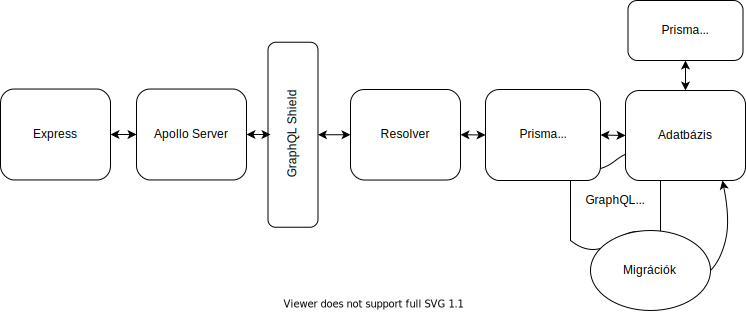
\includegraphics[width=150mm, keepaspectratio]{figures/backend.png}
  \caption{Backend felépítése}
  \label{fig:backend}
\end{figure}

A megfelelő kódrészlet és a middelware-ek futtatása után, a Prismán keresztül az adatbázishoz fordulunk adat lekérés vagy modósítás miatt.

Az ábrán (\refstruc{fig:backend}) világosan látszik, hogy a Prisma által nyújtott studio az adatbázishoz csatlakozik, így az általunk írt üzleti logika nem fog érvenyesülni.
Fontos, hogy az itt végrehajtott modósítások nem várt működéshez is vezethetnek.

%----------------------------------------------------------------------------

\section{Frontend felépítése}

\begin{figure}[!ht]
  \centering
  \includegraphics[width=150mm, keepaspectratio]{figures/frontend.png}
  \caption{Frontend felépítése}
  \label{fig:frontend}
\end{figure}

Ahogy azt a korábbi fejezetekben taglaltam a kliens alkalmazás megvalósításához React-et azon belül pedig NextJS-t használtam.
A backendhez csatlakozást az Apollo Client könyvtárral oldottam meg. 
Az Apollo Client és az Apollo Server együtt egy nagyon jól és könnyen használható rendszert alkotnak.
A Client megkapja a Server-től a GraphQL sémát, így fejlesztés közben kódkiegészítéssel és tipus ellenörzéssel írhatjuk a lekérdezéseinket.
Ezen felül lehetőségünk nyílik kódgenerálásra is.
A megírt GraphQL Query és GraphQL Mutation kódokból React hook-okat kapunk, melyekben az állapot- és a típusokkezelés is megvalósított

%----------------------------------------------------------------------------

\section{Architektúra összefoglalása}
Tehát a három fő komponense az alkalmazásnak a frontend, a backend és az adatbázis.
A frontend és a backend közötti kommunikáció GraphQL segítségével történik az Apollo Cliens és az Apollo Server között.
A backend és az adatbázis kommunikációja pedig SQL segítségével történik, azonban ezt a Prisma teljesen elfedi.

\begin{figure}[!ht]
  \centering
  \includegraphics[width=150mm, keepaspectratio]{figures/architecture.png}
  \caption{Teljes alkalmazás felépítése}
  \label{fig:architecture}
\end{figure}
% !TeX spellcheck = hu_HU
%----------------------------------------------------------------------------
\chapter{Fejlesztést segítő eszközök}
%----------------------------------------------------------------------------
A fejlesztés során igyekeztem minél több olyan eszközt használni, ami elősegíti a munkát és javítja a kódminőséget és biztonságot.
%----------------------------------------------------------------------------

\section{Continuous Integration}
A Continuous Integration napjainkban már elengedhetetlen része a fejlesztési folyamatoknak.
Rengetek megoldás létezik, azonban én a GitHub Action mellett tettem le a voksomat.
Ennek oka, hogy a GitHub–ot használtam a verziókezelt kód tárolására, így kézenfekvő volt ennek a megoldásnak az alkalmazása.

Az alkalmazást 2 külön repository–ban kezeltem, hogy jobban elkülönüljön a frontend és a backend kódja.
Ennek a hátránya az volt, hogy bár ugyan azon nyelvet használja a két repository mégis kétszer kellett implementálnom a GitHub Action–öket.

Az action–ök létrehozását egyszerű szöveges formában tehetjük meg. 
A \lstinline|.github/workflows| mappába létrehozott github \lstinline|.yml| és \lstinline|.yaml| kiterjesztésű fájlok automatikusan kiértékelődnek a GitHub Action által.

\begin{figure}[!ht]
  \centering
  \includegraphics[width=150mm, keepaspectratio]{figures/ci.png}
  \caption{GitHub Action működés közben}
  \label{fig:GitHubAction}
\end{figure}
%----------------------------------------------------------------------------

\subsection{Statikus kódellenőrzés}

\subsubsection{Linter}
A linter egy viszonylag gyors lefutású és kevés erőforrást igénylő action, ezért beállítása szerint bármilyen commit kerül a GitHub repository–ba azonnal lefut és ellenőrzi a kód formázását és jelzi az esetleges hibákat statikus kódellenőrzés segítségével.


%----------------------------------------------------------------------------
\subsubsection{Sercurity check}
A statikus kódellenőrzés egy másik lehetséges felhasználási módja a biztonsági rések keresése, ezt egy a GitHub által ajánlott megoldással valósítottam meg, a CodeQL–lel.
Mivel ez egy több erőforrást igénylő folyamat ezért a futtatása nem történik meg minden commitnál, csak ha az a főágba történik vagy ha Pull Request–et nyit valaki, melynek a cél ága a főág.

A képen (\refstruc{fig:securityCheck}) egy a GitHub által észlelt lehetséges sebezhetőség detektálása látható.
A kód analízis során a rendszer észlelte, hogy shell command futtatása történik úgy, hogy annak tartalma környezeti változóból származik.
A figyelmeztetés jelen esetben egy fals riasztás volt, mert a sérülékeny kódrészlet az alkalmazása futása közben nem érhető el, ugyanis a teszt környezet kialakítására szolgál.

\begin{figure}[!ht]
  \centering
  \includegraphics[width=150mm, keepaspectratio]{figures/security.png}
  \caption{Code scanning figyelmeztetés}
  \label{fig:securityCheck}
\end{figure}
%----------------------------------------------------------------------------

\section{Git hook}
Git használata esetén rengeteg eseményhez definiálhatunk úgynevezett hook–okat.
Ezek segítségével bizonyos események után, előtt vagy közben futtathatunk tetszőleges kódot.
Az alkalmazásomban egy linter–t állítottam be a pre–commit hookra.
Ennek értelmében új commit elkészítése előtt minden alkalommal lefut a linter így biztosítva a kódminőségét.

\begin{lstlisting}[style=ES6, caption=Pre–commit hook beállításai]    
"husky": {
  "hooks": {
    "pre-commit": "lint-staged"
  }
},
"lint-staged": {
  "*.ts": [
    "eslint --fix"
  ]
}
\end{lstlisting}
  
%----------------------------------------------------------------------------

\section{Continuous Delivery}
A Continuous Integration melett elengedhetetlen része a fejlesztésnek a Continuous Delivery.
A CD\footnote{Continuous Delivery} az alkalmazás folyamatos kitelepítését jelenti, hogy a kód felöltése után szinte azonnal elérhető legyen az szoftverünk legfrissebb változata.

%----------------------------------------------------------------------------

\subsection{Heroku}
A backend alkalmazás üzemeltetésére a Heroku szolgáltatásait vettem igénybe.
Webes felületének és GitHub integrációjának köszönhetően nem igényel komoly szakértelmet az alkalmazás elindítása.
Ingyenes keretek között csak egy ág automatikus kitelepítésére van lehetőség, azonban beállítható az is, hogy megvárja a CI\footnote{Continuous Integration} kimenetelét és csak sikeres futás után kezdje el a telepítést.
Így elkerülhetjük hibás– vagy biztonsági réseket tartalmazó kódok éles környezetbe jutását.

%----------------------------------------------------------------------------

\subsection{Vercel}
A frontend üzemeltetéséhez a Vercel–t használtam. 
A Herokuhoz hasonlóan remek GitHub integrációval és webes felülettel rendelkezik. 
Lehetőségünk nyílik a Pull Request–ekhez egy előnézeti alkalmazás kitelepítésére is, ezzel elősegítve a csapatmunkában egymás munkájának ellenőrzését.
Ilyenkor a Vercel automatikusan hozzáad egy megjegyzést (\refstruc{fig:vercel}) a Pull Requesthez az előnézeti alkalmazás linkjével.

\begin{figure}[!ht]
  \centering
  \includegraphics[width=150mm, keepaspectratio]{figures/vercel.png}
  \caption{Vercel megjegyzése Pull Reques–nél}
  \label{fig:vercel}
\end{figure}

%----------------------------------------------------------------------------



%----------------------------------------------------------------------------
\chapter{Alkalmazás fejlesztése}
%----------------------------------------------------------------------------

%----------------------------------------------------------------------------
\section{Backend}
%----------------------------------------------------------------------------


%----------------------------------------------------------------------------
\section{GraphQL séma}
%----------------------------------------------------------------------------


%----------------------------------------------------------------------------
\section{Prisma Studio}
%----------------------------------------------------------------------------


%----------------------------------------------------------------------------
\section{Authentikáció és authorizáció}
%----------------------------------------------------------------------------
GraphQL Shield és JWT


%----------------------------------------------------------------------------
\section{Frontend}
%----------------------------------------------------------------------------

%----------------------------------------------------------------------------
\section{Útvonalválasztás}
%----------------------------------------------------------------------------
NextJS routing

%----------------------------------------------------------------------------
\section{Kódgenerálás}
%----------------------------------------------------------------------------
Apollo codegen

%----------------------------------------------------------------------------
\section{Felhasználói felület}
%----------------------------------------------------------------------------
ChakraUI

%----------------------------------------------------------------------------
\chapter{Tesztelés}
%----------------------------------------------------------------------------

Lorem ipsum

%----------------------------------------------------------------------------
\section{Fronted tesztelés}
%----------------------------------------------------------------------------

Lorem ipsum

%----------------------------------------------------------------------------
\chapter{Üzemeltetés}
%----------------------------------------------------------------------------
\section{Docker}
%----------------------------------------------------------------------------
Az üzemeltetés megkönnyítése érdekében minden komponenshez készítettem egy-egy dockerfile-t és docker-compose file-t.

%----------------------------------------------------------------------------
\section{Deployment}
%----------------------------------------------------------------------------

%----------------------------------------------------------------------------
\chapter{Összefoglalás}
%----------------------------------------------------------------------------

A fejlesztés során rengeteg olyan problémát kellett megoldanom, melyekkel egyébként nem találkoztam volna.
Elmélyültem olyan technologiákban, melyek napjainkban "divatosak" és piaci környezetben is megállják a helyüket.
Ezeket a későbbiekben alkalmazhatom, mint tanulányaimban, mint munkám során.
%----------------------------------------------------------------------------

\section{Tovább fejlesztési lehetőségek}
A félév során temérdek új fejlesztési lehetőség jutott eszembe, melyeket megvalósítva egy még jobb és méginkább a piaci igényeknek megfelelő alkalmazást kaphatunk.
A szakdolgozat keretein belül igyekeztem az elengedhetetlen funkciókat a lehető legjobban megvalósítani és inkább a fejlesztői eszköz tár felépítését tartottam fontosnak, mint a rengeteg funkció belezsúfolását egy alkalmazásba.
Ennek köszönhetően remélhetőleg egy hosszú távon is fejleszthető és fentartható alkalmazás születet.
A félév végeztével folytatnám a munkát, hogy a lehető legtöbb piaci igényt legyen képes kiszolgálni az alkalmazásom.
%----------------------------------------------------------------------------

\subsection{Keresés}
A jelenlegi keresés egy nagyon egyszerű string összehasonlításon alapul, már egyetlen karakter elgépelése esetén sem talál egyezést.
Ennek a problémának a megoldására több lehetőség is kinálkozik, ilyen például az Elastic Search vagy a PostgreSQL-be épített full-text search.
Ezeknek az alapvető működési elve, hogy nem magában az adatbázisban keres hanem létrehoz egy index-szelt szótárat és ezt hasonlítja a keresési kifejezéshez.
Ennek köszönhetően nagy adatbázisok esetén is gyors keresés érhető el.
%----------------------------------------------------------------------------

\subsection{Egyedi tulajdonságok kezelése}
Már a félév elején felvetödött a raktárban tárolt eszközök egyedi tulajdonságainak kezelése, mint ötlet.
A tervezés során kiderült, hogy ez jóval több időt venne igénybe, mint azt az elején gondoltam, így a megvalósítását kihagytam a szakdolgozatból.

A koncepció az volt, hogy kategoriákat hozhattunk volna létre minden raktáron belül.
A kategoriákhoz egy név megadása után felvehetőek lettek volna a tulajdonságok nevei és típusai.
Ezután az eszköz felvételekor kiválasztjuk, hogy milyen kategoriába, kategoriákba tartozik. 
Így a kategoriák révén már tudjuk azt, hogy milyen egyedi tulajdonságai lehetnek.
%----------------------------------------------------------------------------


% List of Figures, Tables
%~~~~~~~~~~~~~~~~~~~~~~~~~~~~~~~~~~~~~~~~~~~~~~~~~~~~~~~~~~~~~~~~~~~~~~~~~~~~~~~~~~~~~~
\listoftables\addcontentsline{toc}{chapter}{\listtablename}


% Bibliography
%~~~~~~~~~~~~~~~~~~~~~~~~~~~~~~~~~~~~~~~~~~~~~~~~~~~~~~~~~~~~~~~~~~~~~~~~~~~~~~~~~~~~~~
\addcontentsline{toc}{chapter}{\bibname}
\bibliography{bib/mybib}


% Appendix
%~~~~~~~~~~~~~~~~~~~~~~~~~~~~~~~~~~~~~~~~~~~~~~~~~~~~~~~~~~~~~~~~~~~~~~~~~~~~~~~~~~~~~~
\include{content/appendices}

%\label{page:last}
\end{document}
